\documentclass[preview]{standalone}

\usepackage{amsmath}
\usepackage{amssymb}
\usepackage{parskip}
\usepackage{fullpage}
\usepackage{hyperref}
\usepackage{tikz}
\usepackage{wrapfig}
\usepackage{bettelini}
\usepackage{stellar}

\hypersetup{
    colorlinks=true,
    linkcolor=black,
    urlcolor=blue,
    pdftitle={Theory of Computation},
    pdfpagemode=FullScreen,
}

\usetikzlibrary{ % tikz packages
    automata,positioning,
    arrows.meta,bending
}

\tikzset{every state/.style={
    inner sep=2pt,
    minimum size=4pt
}}
\tikzset{>=stealth}  %latex, to, stealth

% Empty string symbol.
\newcommand{\emptyString}{\lambda}

\begin{document}

\title{Theory of Computation}
\id{theoryofcomputation}
\genpage

%%%%%%%

\section{Regular Expressions}

A regular expression is a mean to express a language.
The class of languages that can be described by
regular expressions coincides with the class of regular languages.

\section{Properties}

Let \(R_1\) be a regular expression describing \(L_1\) and \(R_2\) a regular expression
describing \(L_2\).

\begin{itemize}
    \item \(\emptyString\) is a regular expression describing  \(\{\emptyString\}\)
    \item \(\emptyset\) is a regular expression describing \(\emptyset\)
    \item \(\emptyset^*\) is a regular expression describing \(\{\emptyString\}\)
    \item Let \(\Sigma\) be a non-empty alphabet, \(\forall a \in \Sigma, a\) is a regular expression describing \(\{a\}\)
    \item \(R_1R_2\) is a regular expression describing \(L_1L_2\)
    \item \(R_1\union R_2\) is a regular expression describing \(L_1\union L_2\)
    \item \(R_1\intersection R_2\) is a regular expression describing \(L_1\intersection L_2\)
    \item \(R_1^*\) is a regular expression describing \(L_1^*\)
    \item \(\bar{R_1}\) is a regular expression describing \(\bar{L_1}\)
\end{itemize}
If \(L_1 = L_2\), then we say \(R_1 = R_2\) (e.g. \(\emptyString = \emptyset^*\)).

Let \(R_1, R_2\) and \(R_3\) be regular expressions
\begin{itemize}
    \item \(R_1 \emptyset = \emptyset R_1 = \emptyset\)
    \item \(R_1 \emptyString = \emptyString R_1 = R_1\)
    \item \(R_1 \union R_2 = R_2 \union R_1\)
    \item \(R_1 \union \emptyset = R_1\)
    \item \(R_1 \union R_1 = R_1\)
    \item \(R_1(R_2 \union R_3) = R_1R_2 \union R_1R_3\)
    \item \((R_1 \union R_2)R_3 = R_1R_3 \union R_2R_3\)
    \item \(R_1(R_2R_3) = (R_1R_2)R_3\)
    \item \(\emptyset^*=\emptyString\)
    \item \(\emptyString^*=\emptyString\)
    \item \((\emptyString \union R_1)^* = R_1^*\)
    \item \((\emptyString \union R_1)(\emptyString \union R_1)^* = R_1^*\)
    \item \(R_1^*(\emptyString \union R_1)=(\emptyString \union R_1)R_1^* = R_1^*\)
    \item \(R_1^*R_2 \union R_2 = R_1^*R_2\)
    \item \(R_1(R_2R_1)^*=(R_1R_2)^*R_1\)
    \item \((R_1 \union R_2)^* = (R_1^*R_2)^*R_1^* = (R_2^*R_1)^*R_2^*\)
\end{itemize}

\section{Equivalence of regular expressions and regular languages}

\subsection{A regular expression describes a regular language}

Let \(R\) be a regular expression over \(\Sigma\).

\begin{wrapfigure}{r}{2.5cm}
    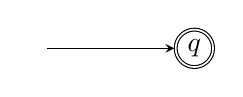
\begin{tikzpicture}[node distance=2cm,on grid,auto]
        \node[state, accepting] (q) {\(q\)};
        \node (inv) [left=of q] {};
    
        \path[->]
            (inv)
                edge node {} (q);
    \end{tikzpicture}
\end{wrapfigure}

Assume that \(R=\emptyString\). Then \(R\) describes \(\{\emptyString\}\).
This language is regular and we can prove it by constructing an NFA \(N=(Q, \Sigma, \delta, q, F)\)
such that \(L(N)=\{\emptyString\}\).
\(q\) is the start state, \(Q=\{q\}\), \(F=\{q\}\) and \(\delta(r,a)=\emptyset\)
where \(a\in\Sigma_\emptyString\).
\wrapfill

\begin{wrapfigure}{r}{2.5cm}
    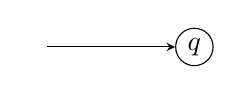
\begin{tikzpicture}[node distance=2cm,on grid,auto]
        \node[state] (q) {\(q\)};
        \node (inv) [left=of q] {};
    
        \path[->]
            (inv)
                edge node {} (q);
    \end{tikzpicture}
\end{wrapfigure}

Assume that \(R=\emptyset\). Then \(R\) describes \(\emptyset\).
This language is regular and we can prove it by constructing an NFA \(N=(Q, \Sigma, \delta, q, F)\)
such that \(L(N)=\emptyset\).
\(q\) is the start state, \(Q=\{q\}\), \(F=\emptyset\) and \(\delta(r,a)=\emptyset\) where \(a\in\Sigma_\emptyString\).
\wrapfill

\begin{wrapfigure}{r}{2.5cm}
    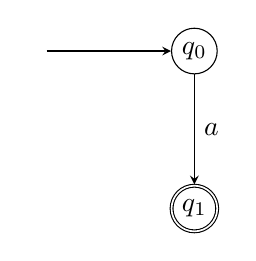
\begin{tikzpicture}[node distance=2cm,on grid,auto]
        \node (inv) {};
        \node[state] (q0) [right=of inv] {\(q_0\)};
        \node[state, accepting] (q1) [below=of q0] {\(q_1\)};
    
        \path[->]
            (inv)
                edge node {} (q0)
            (q0)
                edge node {\(a\)} (q1);
    \end{tikzpicture}
\end{wrapfigure}

Assume that \(R=a\) where \(a\in\Sigma\). Then \(R\) describes \(\{a\}\).
This language is regular and we can prove it by constructing an NFA \(N=(Q, \Sigma, \delta, q, F)\)
such that \(L(N)=\{a\}\).
\(q_0\) is the start state, \(Q=\{q_0, q_1\}\), \(F=\{q_1\}\) and
\[
    \delta(r,b \in) =
    \begin{cases}
        \{q_1\} & b=a \land r=q_0\\
        \emptyset & \text{otherwise}
    \end{cases}
\]
where \(b\in\Sigma_\emptyString\).
\wrapfill

Assume that \(R=R_1 \union R_2\) where \(R_1\) and \(R_2\) are regular expressions.
Let \(L_1\) and \(L_2\) be the languages described by \(R_1\) and \(R_2\) respectively.
Assuming that \(L_1\) and \(L_2\) are regular, \(R\) then describes \(L_1 \union L_2\) which by theorem is regular.

Assume that \(R=R_1 \intersection R_2\) where \(R_1\) and \(R_2\) are regular expressions.
Let \(L_1\) and \(L_2\) be the languages described by \(R_1\) and \(R_2\) respectively.
Assuming that \(L_1\) and \(L_2\) are regular, \(R\) then describes \(L_1 \intersection L_2\) which by theorem is regular.

Assume that \(R=R_1 R_2\) where \(R_1\) and \(R_2\) are regular expressions.
Let \(L_1\) and \(L_2\) be the languages described by \(R_1\) and \(R_2\) respectively.
Assuming that \(L_1\) and \(L_2\) are regular, \(R\) then describes \(L_1 L_2\) which by theorem is regular.

Assume that \(R={(R_1)}^*\) where \(R_1\) is a regular expression. Let \(L_1\) be the language be described
by \(R_1\). Assuming that \(L_1\) is regular, then \(R\) describes \({(L_1)}^*\) which by theorem is regular.

Assume that \(R=\bar{R_1}\) where \(R_1\) is a regular expression. Let \(L_1\) be the language be described
by \(R_1\). Assuming that \(L_1\) is regular, then \(R\) describes \(\bar{L_1}\) which by theorem is regular.

This proves that every regular expression describes a regular language since every
regular expression can be broken down to regular languages.

\subsection{A DFA can be converted into a regular expression}

\subsubsection{Solving recurrence relations}

Let \(\Sigma\) be an alphabet and let \(B\), \(C\) and \(L\) be languages in \(\Sigma^*\) where \(\emptyString \notin B\)
\[
    L=BL\union C \implies L=B^*C
\]

In order to prove this we first show that \(B^*C \subseteq L\) by induction.
Let \(w \in B^*C\), then \(w\) is \(k\geq 0\) strings in \(B\) followed a string in \(C\).
When \(k=0\), \(w \in C\) which implies \(w \in BL\union C\) which implies \(w \in L\).
When \(k > 0\) we can write \(w\) as \(xyz\) where \(x\) is a string in \(B\),
\(y\) is the concatenation of \(k-1\) strings in \(B\) and \(c \in C\).
Let \(q=yz\). Since \(q\) is a concatenation of \(k-1\) strings of \(B\) followed by a string in \(C\),
\(q \in L\). Hence, \(w=xq\) where \(x\in B\) and \(q\in L\). This shows that \(w \in BL\).
Hence, \(w \in BL\union C\). Since \(BL \union C = L\), \(w \in L\). This proves that
\(B^*C\subseteq L\). \\
Now we show that \(L \subseteq B^*C\) by induction to conclude the proof.
Let \(w\in L\). When \(|w|=0\), \(w=\emptyString\). Since \(\emptyString \notin B\),
\(w \notin BL\). This means that \(w\in C\). Since \(C \subseteq B^*C\) the string \(w\)
is also in \(B^*C\). When \(|w| > 0\), if \(w \in C\) then \(w \in B^*C\),
If \(w \notin C\), \(w \in BL\) since \(w \in L\) and \(L=BL\union C\).
Hence, \(w=bl\) where \(b\in B\) and \(l\in L\).
Since \(\emptyString \notin B\), \(|b|>0\). This means that \(|l|<|b|\)
since \(|l|+|b|=|w|\). By induction, \(l\) is a string in \(B^*C\).
Hence, \(w = bl\) where \(b\in B\) and \(l\in B^*C\). This shows that \(w \in B(B^*C)\).
Since \(B(B^*C) \subseteq B^*C\) it follows that \(w \in B^*C\).

\subsubsection{The conversion}

We will now prove that every DFA can be converted into a regular expression.
Let \(M=(Q, \Sigma, \delta, q, F)\) be a DFA. We will prove that there exists a regular
expression describing \(L(M)\).

We define \(L_r\) where \(r \in Q\) as the set of strings \(w \in \Sigma_\emptyString\)
that would be accepted by \(M\) if \(r\) were its start state, meaning the language of \(M\)
if \(r\) were its start state. Note that \(L(M)=L_q\).

\subsection{Conclusion}

Since any DFA \(M\) can be converted into a regular expression that describes \(L(M)\)
and every regular expression describes a regular language, we can conclude that a language \(L\)
is regular if there exists a regular expression that describes \(L\).

\end{document}